
%% bare_conf.tex
%% V1.4b
%% 2015/08/26
%% by Michael Shell
%% See:
%% http://www.michaelshell.org/
%% for current contact information.
%%
%% This is a skeleton file demonstrating the use of IEEEtran.cls
%% (requires IEEEtran.cls version 1.8b or later) with an IEEE
%% conference paper.
%%
%% Support sites:
%% http://www.michaelshell.org/tex/ieeetran/
%% http://www.ctan.org/pkg/ieeetran
%% and
%% http://www.ieee.org/

%%*************************************************************************
%% Legal Notice:
%% This code is offered as-is without any warranty either expressed or
%% implied; without even the implied warranty of MERCHANTABILITY or
%% FITNESS FOR A PARTICULAR PURPOSE! 
%% User assumes all risk.
%% In no event shall the IEEE or any contributor to this code be liable for
%% any damages or losses, including, but not limited to, incidental,
%% consequential, or any other damages, resulting from the use or misuse
%% of any information contained here.
%%
%% All comments are the opinions of their respective authors and are not
%% necessarily endorsed by the IEEE.
%%
%% This work is distributed under the LaTeX Project Public License (LPPL)
%% ( http://www.latex-project.org/ ) version 1.3, and may be freely used,
%% distributed and modified. A copy of the LPPL, version 1.3, is included
%% in the base LaTeX documentation of all distributions of LaTeX released
%% 2003/12/01 or later.
%% Retain all contribution notices and credits.
%% ** Modified files should be clearly indicated as such, including  **
%% ** renaming them and changing author support contact information. **
%%*************************************************************************


% *** Authors should verify (and, if needed, correct) their LaTeX system  ***
% *** with the testflow diagnostic prior to trusting their LaTeX platform ***
% *** with production work. The IEEE's font choices and paper sizes can   ***
% *** trigger bugs that do not appear when using other class files.       ***                          ***
% The testflow support page is at:
% http://www.michaelshell.org/tex/testflow/



\documentclass[conference, letterpaper]{IEEEtran}
% Some Computer Society conferences also require the compsoc mode option,
% but others use the standard conference format.
%
% If IEEEtran.cls has not been installed into the LaTeX system files,
% manually specify the path to it like:
% \documentclass[conference]{../sty/IEEEtran}





% Some very useful LaTeX packages include:
% (uncomment the ones you want to load)


% *** MISC UTILITY PACKAGES ***
%
%\usepackage{ifpdf}
% Heiko Oberdiek's ifpdf.sty is very useful if you need conditional
% compilation based on whether the output is pdf or dvi.
% usage:
% \ifpdf
%   % pdf code
% \else
%   % dvi code
% \fi
% The latest version of ifpdf.sty can be obtained from:
% http://www.ctan.org/pkg/ifpdf
% Also, note that IEEEtran.cls V1.7 and later provides a builtin
% \ifCLASSINFOpdf conditional that works the same way.
% When switching from latex to pdflatex and vice-versa, the compiler may
% have to be run twice to clear warning/error messages.






% *** CITATION PACKAGES ***
%
\usepackage{cite}
% cite.sty was written by Donald Arseneau
% V1.6 and later of IEEEtran pre-defines the format of the cite.sty package
% \cite{} output to follow that of the IEEE. Loading the cite package will
% result in citation numbers being automatically sorted and properly
% "compressed/ranged". e.g., [1], [9], [2], [7], [5], [6] without using
% cite.sty will become [1], [2], [5]--[7], [9] using cite.sty. cite.sty's
% \cite will automatically add leading space, if needed. Use cite.sty's
% noadjust option (cite.sty V3.8 and later) if you want to turn this off
% such as if a citation ever needs to be enclosed in parenthesis.
% cite.sty is already installed on most LaTeX systems. Be sure and use
% version 5.0 (2009-03-20) and later if using hyperref.sty.
% The latest version can be obtained at:
% http://www.ctan.org/pkg/cite
% The documentation is contained in the cite.sty file itself.






% *** GRAPHICS RELATED PACKAGES ***
%
\ifCLASSINFOpdf
  \usepackage[pdftex]{graphicx}
  % declare the path(s) where your graphic files are
  \graphicspath{{../fig/}}
  % and their extensions so you won't have to specify these with
  % every instance of \includegraphics
  \DeclareGraphicsExtensions{.pdf,.jpeg,.png}
\else
  % or other class option (dvipsone, dvipdf, if not using dvips). graphicx
  % will default to the driver specified in the system graphics.cfg if no
  % driver is specified.
  % \usepackage[dvips]{graphicx}
  % declare the path(s) where your graphic files are
  % \graphicspath{{../eps/}}
  % and their extensions so you won't have to specify these with
  % every instance of \includegraphics
  % \DeclareGraphicsExtensions{.eps}
\fi
% graphicx was written by David Carlisle and Sebastian Rahtz. It is
% required if you want graphics, photos, etc. graphicx.sty is already
% installed on most LaTeX systems. The latest version and documentation
% can be obtained at: 
% http://www.ctan.org/pkg/graphicx
% Another good source of documentation is "Using Imported Graphics in
% LaTeX2e" by Keith Reckdahl which can be found at:
% http://www.ctan.org/pkg/epslatex
%
% latex, and pdflatex in dvi mode, support graphics in encapsulated
% postscript (.eps) format. pdflatex in pdf mode supports graphics
% in .pdf, .jpeg, .png and .mps (metapost) formats. Users should ensure
% that all non-photo figures use a vector format (.eps, .pdf, .mps) and
% not a bitmapped formats (.jpeg, .png). The IEEE frowns on bitmapped formats
% which can result in "jaggedy"/blurry rendering of lines and letters as
% well as large increases in file sizes.
%
% You can find documentation about the pdfTeX application at:
% http://www.tug.org/applications/pdftex





% *** MATH PACKAGES ***
%
%\usepackage{amsmath}
% A popular package from the American Mathematical Society that provides
% many useful and powerful commands for dealing with mathematics.
%
% Note that the amsmath package sets \interdisplaylinepenalty to 10000
% thus preventing page breaks from occurring within multiline equations. Use:
%\interdisplaylinepenalty=2500
% after loading amsmath to restore such page breaks as IEEEtran.cls normally
% does. amsmath.sty is already installed on most LaTeX systems. The latest
% version and documentation can be obtained at:
% http://www.ctan.org/pkg/amsmath





% *** SPECIALIZED LIST PACKAGES ***
%
%\usepackage{algorithmic}
% algorithmic.sty was written by Peter Williams and Rogerio Brito.
% This package provides an algorithmic environment fo describing algorithms.
% You can use the algorithmic environment in-text or within a figure
% environment to provide for a floating algorithm. Do NOT use the algorithm
% floating environment provided by algorithm.sty (by the same authors) or
% algorithm2e.sty (by Christophe Fiorio) as the IEEE does not use dedicated
% algorithm float types and packages that provide these will not provide
% correct IEEE style captions. The latest version and documentation of
% algorithmic.sty can be obtained at:
% http://www.ctan.org/pkg/algorithms
% Also of interest may be the (relatively newer and more customizable)
% algorithmicx.sty package by Szasz Janos:
% http://www.ctan.org/pkg/algorithmicx




% *** ALIGNMENT PACKAGES ***
%
%\usepackage{array}
% Frank Mittelbach's and David Carlisle's array.sty patches and improves
% the standard LaTeX2e array and tabular environments to provide better
% appearance and additional user controls. As the default LaTeX2e table
% generation code is lacking to the point of almost being broken with
% respect to the quality of the end results, all users are strongly
% advised to use an enhanced (at the very least that provided by array.sty)
% set of table tools. array.sty is already installed on most systems. The
% latest version and documentation can be obtained at:
% http://www.ctan.org/pkg/array


% IEEEtran contains the IEEEeqnarray family of commands that can be used to
% generate multiline equations as well as matrices, tables, etc., of high
% quality.




% *** SUBFIGURE PACKAGES ***
%\ifCLASSOPTIONcompsoc
%  \usepackage[caption=false,font=normalsize,labelfont=sf,textfont=sf]{subfig}
%\else
%  \usepackage[caption=false,font=footnotesize]{subfig}
%\fi
% subfig.sty, written by Steven Douglas Cochran, is the modern replacement
% for subfigure.sty, the latter of which is no longer maintained and is
% incompatible with some LaTeX packages including fixltx2e. However,
% subfig.sty requires and automatically loads Axel Sommerfeldt's caption.sty
% which will override IEEEtran.cls' handling of captions and this will result
% in non-IEEE style figure/table captions. To prevent this problem, be sure
% and invoke subfig.sty's "caption=false" package option (available since
% subfig.sty version 1.3, 2005/06/28) as this is will preserve IEEEtran.cls
% handling of captions.
% Note that the Computer Society format requires a larger sans serif font
% than the serif footnote size font used in traditional IEEE formatting
% and thus the need to invoke different subfig.sty package options depending
% on whether compsoc mode has been enabled.
%
% The latest version and documentation of subfig.sty can be obtained at:
% http://www.ctan.org/pkg/subfig




% *** FLOAT PACKAGES ***
%
%\usepackage{fixltx2e}
% fixltx2e, the successor to the earlier fix2col.sty, was written by
% Frank Mittelbach and David Carlisle. This package corrects a few problems
% in the LaTeX2e kernel, the most notable of which is that in current
% LaTeX2e releases, the ordering of single and double column floats is not
% guaranteed to be preserved. Thus, an unpatched LaTeX2e can allow a
% single column figure to be placed prior to an earlier double column
% figure.
% Be aware that LaTeX2e kernels dated 2015 and later have fixltx2e.sty's
% corrections already built into the system in which case a warning will
% be issued if an attempt is made to load fixltx2e.sty as it is no longer
% needed.
% The latest version and documentation can be found at:
% http://www.ctan.org/pkg/fixltx2e


%\usepackage{stfloats}
% stfloats.sty was written by Sigitas Tolusis. This package gives LaTeX2e
% the ability to do double column floats at the bottom of the page as well
% as the top. (e.g., "\begin{figure*}[!b]" is not normally possible in
% LaTeX2e). It also provides a command:
%\fnbelowfloat
% to enable the placement of footnotes below bottom floats (the standard
% LaTeX2e kernel puts them above bottom floats). This is an invasive package
% which rewrites many portions of the LaTeX2e float routines. It may not work
% with other packages that modify the LaTeX2e float routines. The latest
% version and documentation can be obtained at:
% http://www.ctan.org/pkg/stfloats
% Do not use the stfloats baselinefloat ability as the IEEE does not allow
% \baselineskip to stretch. Authors submitting work to the IEEE should note
% that the IEEE rarely uses double column equations and that authors should try
% to avoid such use. Do not be tempted to use the cuted.sty or midfloat.sty
% packages (also by Sigitas Tolusis) as the IEEE does not format its papers in
% such ways.
% Do not attempt to use stfloats with fixltx2e as they are incompatible.
% Instead, use Morten Hogholm'a dblfloatfix which combines the features
% of both fixltx2e and stfloats:
%
% \usepackage{dblfloatfix}
% The latest version can be found at:
% http://www.ctan.org/pkg/dblfloatfix




% *** PDF, URL AND HYPERLINK PACKAGES ***
%
%\usepackage{url}
% url.sty was written by Donald Arseneau. It provides better support for
% handling and breaking URLs. url.sty is already installed on most LaTeX
% systems. The latest version and documentation can be obtained at:
% http://www.ctan.org/pkg/url
% Basically, \url{my_url_here}.




% *** Do not adjust lengths that control margins, column widths, etc. ***
% *** Do not use packages that alter fonts (such as pslatex).         ***
% There should be no need to do such things with IEEEtran.cls V1.6 and later.
% (Unless specifically asked to do so by the journal or conference you plan
% to submit to, of course. )


% correct bad hyphenation here
\hyphenation{op-tical net-works semi-conduc-tor}

\usepackage[utf8]{inputenc}

\begin{document}
%
% paper title
% Titles are generally capitalized except for words such as a, an, and, as,
% at, but, by, for, in, nor, of, on, or, the, to and up, which are usually
% not capitalized unless they are the first or last word of the title.
% Linebreaks \\ can be used within to get better formatting as desired.
% Do not put math or special symbols in the title.
\title{Improvement of Visual Servoing Tasks by Underwater Image Enhancement}


% author names and affiliations
% use a multiple column layout for up to three different
% affiliations
\author{
    \IEEEauthorblockN{
    Diego Cesar\IEEEauthorrefmark{1},
    Sylvain Joyeux\IEEEauthorrefmark{1},
    Marco Reis\IEEEauthorrefmark{1},
    André Conceição\IEEEauthorrefmark{2},
    Jan Albiez\IEEEauthorrefmark{1}
    }
	\IEEEauthorblockA{\IEEEauthorrefmark{1}Brazilian Institute of Robotics, SENAI 
	CIMATEC, Salvador, Bahia, Brazil}
	\IEEEauthorblockA{\IEEEauthorrefmark{2}Electrical Engineering Department,, UFBA, 
    Salvador, Bahia, Brazil \\ Email: diego.cesar@fieb.org.br}
}
% conference papers do not typically use \thanks and this command
% is locked out in conference mode. If really needed, such as for
% the acknowledgment of grants, issue a \IEEEoverridecommandlockouts
% after \documentclass

% for over three affiliations, or if they all won't fit within the width
% of the page, use this alternative format:
% 
%\author{\IEEEauthorblockN{Michael Shell\IEEEauthorrefmark{1},
%Homer Simpson\IEEEauthorrefmark{2},
%James Kirk\IEEEauthorrefmark{3}, 
%Montgomery Scott\IEEEauthorrefmark{3} and
%Eldon Tyrell\IEEEauthorrefmark{4}}
%\IEEEauthorblockA{\IEEEauthorrefmark{1}School of Electrical and Computer Engineering\\
%Georgia Institute of Technology,
%Atlanta, Georgia 30332--0250\\ Email: see http://www.michaelshell.org/contact.html}
%\IEEEauthorblockA{\IEEEauthorrefmark{2}Twentieth Century Fox, Springfield, USA\\
%Email: homer@thesimpsons.com}
%\IEEEauthorblockA{\IEEEauthorrefmark{3}Starfleet Academy, San Francisco, California 96678-2391\\
%Telephone: (800) 555--1212, Fax: (888) 555--1212}
%\IEEEauthorblockA{\IEEEauthorrefmark{4}Tyrell Inc., 123 Replicant Street, Los Angeles, California 90210--4321}}




% use for special paper notices
%\IEEEspecialpapernotice{(Invited Paper)}




% make the title area
\maketitle

% As a general rule, do not put math, special symbols or citations
% in the abstract
\begin{abstract}

Underwater image formation is degraded by several factors, which causes the
    ocean to be a challenging environment for image processing. This paper aims
    to improve the visual servoing capability of an autonomous underwater
    vehicle by using pre-processing algorithms to improve the image quality.
    We used artificial fiducial markers to feed the visual controller.
    Therefore, three different methods for imaging enhancing were applied to the
    raw image aiming to increase the detection rate of the marker detector.
    Since the performance of the visual controller also depends on the
    detection time, this variable was also considered in the comparison.
    Finally, the algorithm that caused the best improvement in marker
    detection was tested in a visual servoing mission. The proposed methods
    have shown a significantly improvement in the marker detection rates at
    reasonable detection times for visual servoing of autonomous underwater
    vehicles. In terms of visual servoing missions, this work shows that the
    proposed methods not only increased the controller frequency, but also made
    visual servoing possible when water condition is not favorable and no
    marker can be detected without a pre-processing layer.
\end{abstract}

% no keywords




% For peer review papers, you can put extra information on the cover
% page as needed:
% \ifCLASSOPTIONpeerreview
% \begin{center} \bfseries EDICS Category: 3-BBND \end{center}
% \fi
%
% For peerreview papers, this IEEEtran command inserts a page break and
% creates the second title. It will be ignored for other modes.
%\IEEEpeerreviewmaketitle



\section{Introduction}\label{sec:int}

Underwater image analysis is useful for many applications, such as:
inspection of man-made structures, observation of marine fauna, monitoring,
seabed studies \cite{Aulinas2011}. Nonetheless, unlike normal images taken in
the air, the physical characteristics of the water medium causes underwater
images to be usually affected by limited range visibility, low contrast, non
uniform lighting, blurring, bright artifacts, and noise \cite{Yang2012}.

Light attenuation in water is caused by light absorption and light
scattering. The former reduces the energy of light while the latter changes the
direction of the light. It directly affects light visibility, which can vary
from twenty up to five meters or even less \cite{Schettini2010}. Light
attenuation is not caused only by light propagation in the water medium, but
also due to dissolved and floating particles in the water. These
interactions increase absorption and scattering effects.

Thus, several works have been published aiming to make underwater images more
comprehensible to humans and even for machines, since it would permit the use
of standard image processing algorithms \cite{Schettini2010} \cite{sankpal2016nonuniform} \cite{rodrigues2016enhancement} \cite{bazeille2006automatic}
\cite{arnold2005preprocessing} \cite{chiang2012underwater} \cite{iqbal2007underwater}.

One of the multiple interests in improving underwater image quality is
feature extraction for visual servoing. Visual servoing or vision-based
control is a control scheme that uses visual information to control the motion
of a robot. It is a multidisciplinary field that covers the knowledge of areas
such as kinematics, dynamics, image processing and control theory
\cite{Hutchinson1996}. Visual servoing mimics the way that humans use their
visual system to perform simple actions such as grabbing objects, positioning
the body to enter through a door or seating on a chair. On underwater robots,
visual servoing can be useful for performing tasks such as docking
\cite{Lee2003}, pipeline following \cite{Rives1997} and structure inspection
\cite{KRUPINSKI2015274}. Moreover, underwater visual servoing has been used
for aiding robot inspection and 3D reconstruction \cite{4302315}, assisting
ROV pilots \cite{4099090} and valves manipulation \cite{1282820}.

As visual servoing relies on the feature extraction, this work will take
advantage of the artificial fiducial markers. They are patterns that encode
unique ID and are especially designed to be easily detected by computer vision
systems. In Figure \ref{fig:marker_systems} some fiducial marker systems are
shown.

\begin{figure}[!ht]
	\centering
    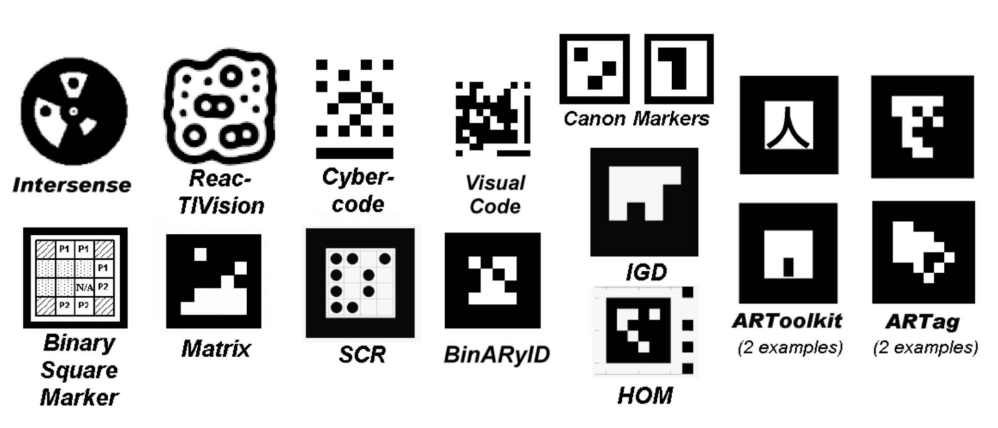
\includegraphics[width=0.40\textwidth]{./fig/marker_systems.png}
    \caption[Different marker systems]{Different marker systems \cite{Fiala2010}}
	\label{fig:marker_systems}
\end{figure}

Given these characteristics, artificial fiducial markers have high detection
and low false-positive and false-negative rates. The use of fiducial markers is
suitable when object recognition or pose determination is needed with high
reliability and when the environment can be modified to affix them \cite{Fiala2010}. 

This paper quantitatively compares three different approaches for underwater
image enhancement, taking in account the marker detection rate and processing
time. It shows how the use of an image pre-processing layer can significantly
increase the detection rate of the marker detector, improving the performance
of a vehicle servoing in front of a marker.

The document is divided in Section \ref{sec:int}, which shows the state of the art
and the paper goal, Section \ref{sec:exp_proced} shows the experimental
procedures and details the applied methods, Section \ref{sec:results} shows the
achieved results and discusses them and Section \ref{sec:concl} presents the
conclusion of this work.

\section{Experimental Procedures} \label{sec:exp_proced}

In order to evaluate the different proposed methods, we used FlatFish AUV (Figure
\ref{fig:flatfish_1}) \cite{flatfish_jan} to collect data to be analyzed
offline. FlatFish is an AUV developed by the Brazilian Institute of Robotics
and the Robotics Innovation Center as part of the FlatFish project, a project
founded by Shell which aims to develop an AUV for inspection of assets from O\&G industry.

\begin{figure}[!ht]
    \centering
    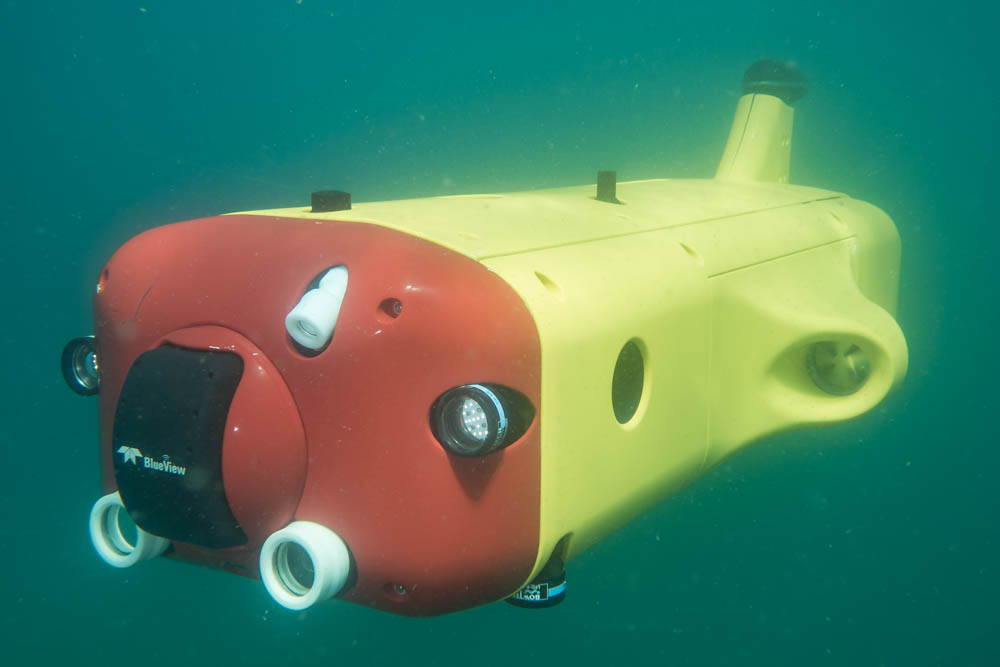
\includegraphics[width=0.45\textwidth]{./fig/20160317-FF-Test-P1040442.jpg}
    \caption{FlatFish AUV.}
    \label{fig:flatfish_1}
\end{figure}

In the context of this work, it is important to mention that FlatFish is
equipped with four cameras Basler acA2040-gc25, able to capture up to 25 frames
per second with 2040 x 2040 resolution. The actuation system is composed of 6
thrusters disposed according to Figure \ref{fig:thrusters_configuration}. This
configuration controls 4 degrees of freedom, where roll and pitch are passively
controlled. 

\begin{figure}[!ht]
    \centering
    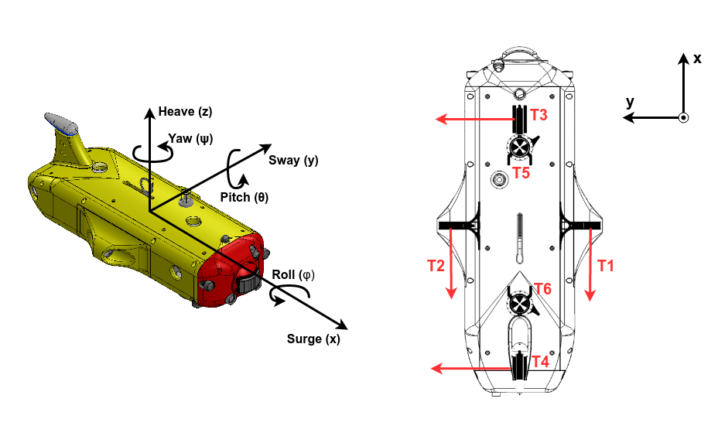
\includegraphics[width=0.45\textwidth]{./fig/thrust_configuration.png}
    \caption{FlatFish thruster configuration \cite{saback2016}.}
    \label{fig:thrusters_configuration}
\end{figure}

The experiments were conducted in the Todos os Santos Bay, located in the city
of Salvador-BA, part of the Brazilian coast. A marker attached to an iron
pedestal was deployed in shallow waters, 20 meters deep. The vehicle was
placed in front of the marker, changing its marker-relative pose in terms of
position and orientation. At the end, one hour video containing 32613 frames was
acquired for posteriori analysis. Apriltags marker system was chosen due
to having presented the best performance among the open-source libraries
\cite{diego}.  Figure \ref{fig:apriltag_pedestal} shows the detection of
Apriltags in the ocean.

\begin{figure}[!htpb]
	\centering
	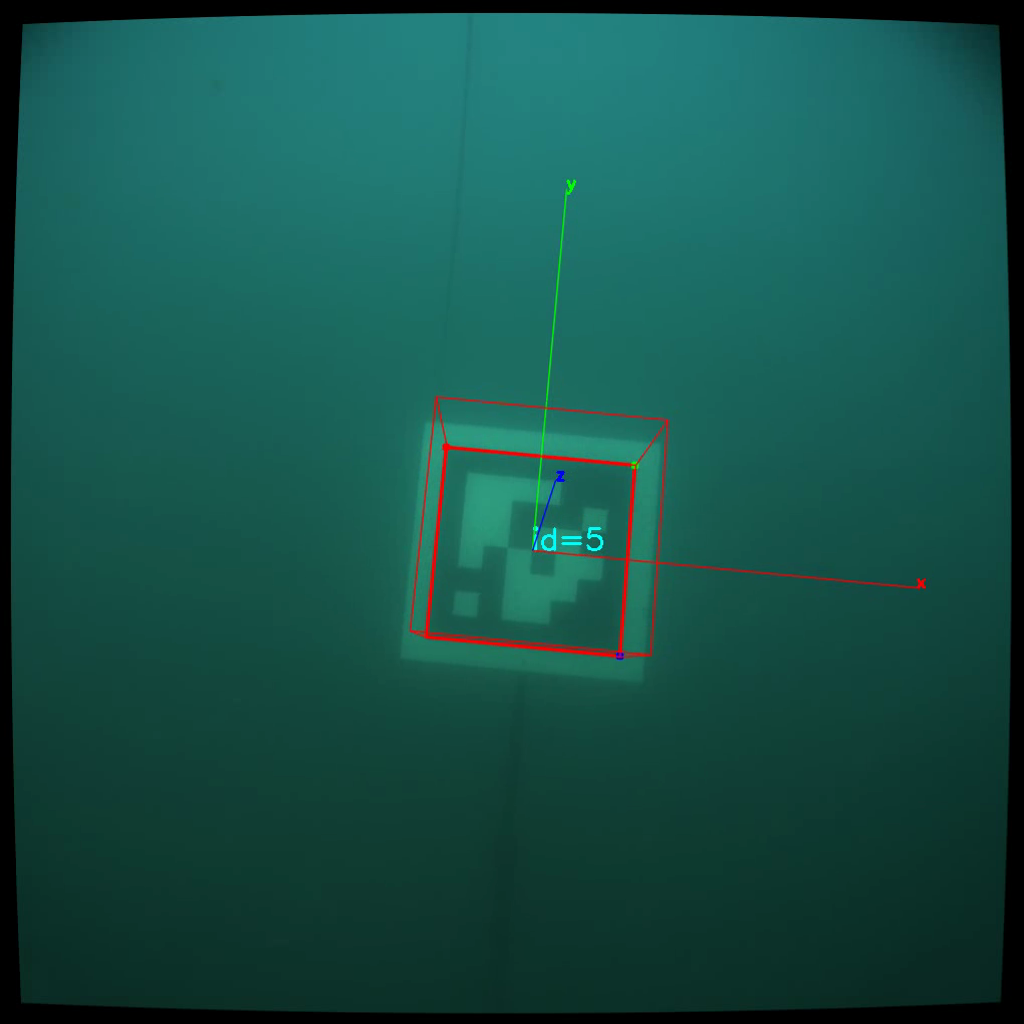
\includegraphics[width=0.45\textwidth]{./fig/april_ocean3.png}
    \caption{Vehicle's camera detecting the Apriltag marker.}
    \label{fig:apriltags_ocean}
\end{figure}

The experiment consisted in performing the pre-processing algorithms on the
entire video and comparing which one of the methods gave the highest detection
rate. Since the detected frames feed a visual controller, the time for
detection is also a relevant factor. Therefore, we also downscaled images and
observed how this affected the processing time. Acquired image resolution was
2040x2040 and in this work it was scaled by the following factors: 0.5 0.4 0.3 0.2
0.1 0.05.

\subsection{Methods}

The pre-processing algorithms in which the raw image was submitted is here described. 

The first approach, namely Method 1, converts the raw image to grayscale
before sending it to the Apriltag detector. Method 2 adds a stage of
normalization as a simple contrast stretching stage. Method 3 is similar to
Method 2, although it uses contrast limited adaptive histogram equalization (CLAHE)
\cite{zuiderveld1994contrast} to improve the contrast of the grayscale image.
Method 4 is based on the method proposed by Iqbal \cite{iqbal2007underwater},
with the differences that we used HSV instead of HSI and the contrast stretching was
also performed locally using CLAHE, as opposed to the method proposed by
the authors.

Figure \ref{fig:methods_flow} shows a diagram with the pre-processing stages
applied to the raw image before it was processed by the marker detector, for each
method. 

\begin{figure}[!htpb]
    \centering
    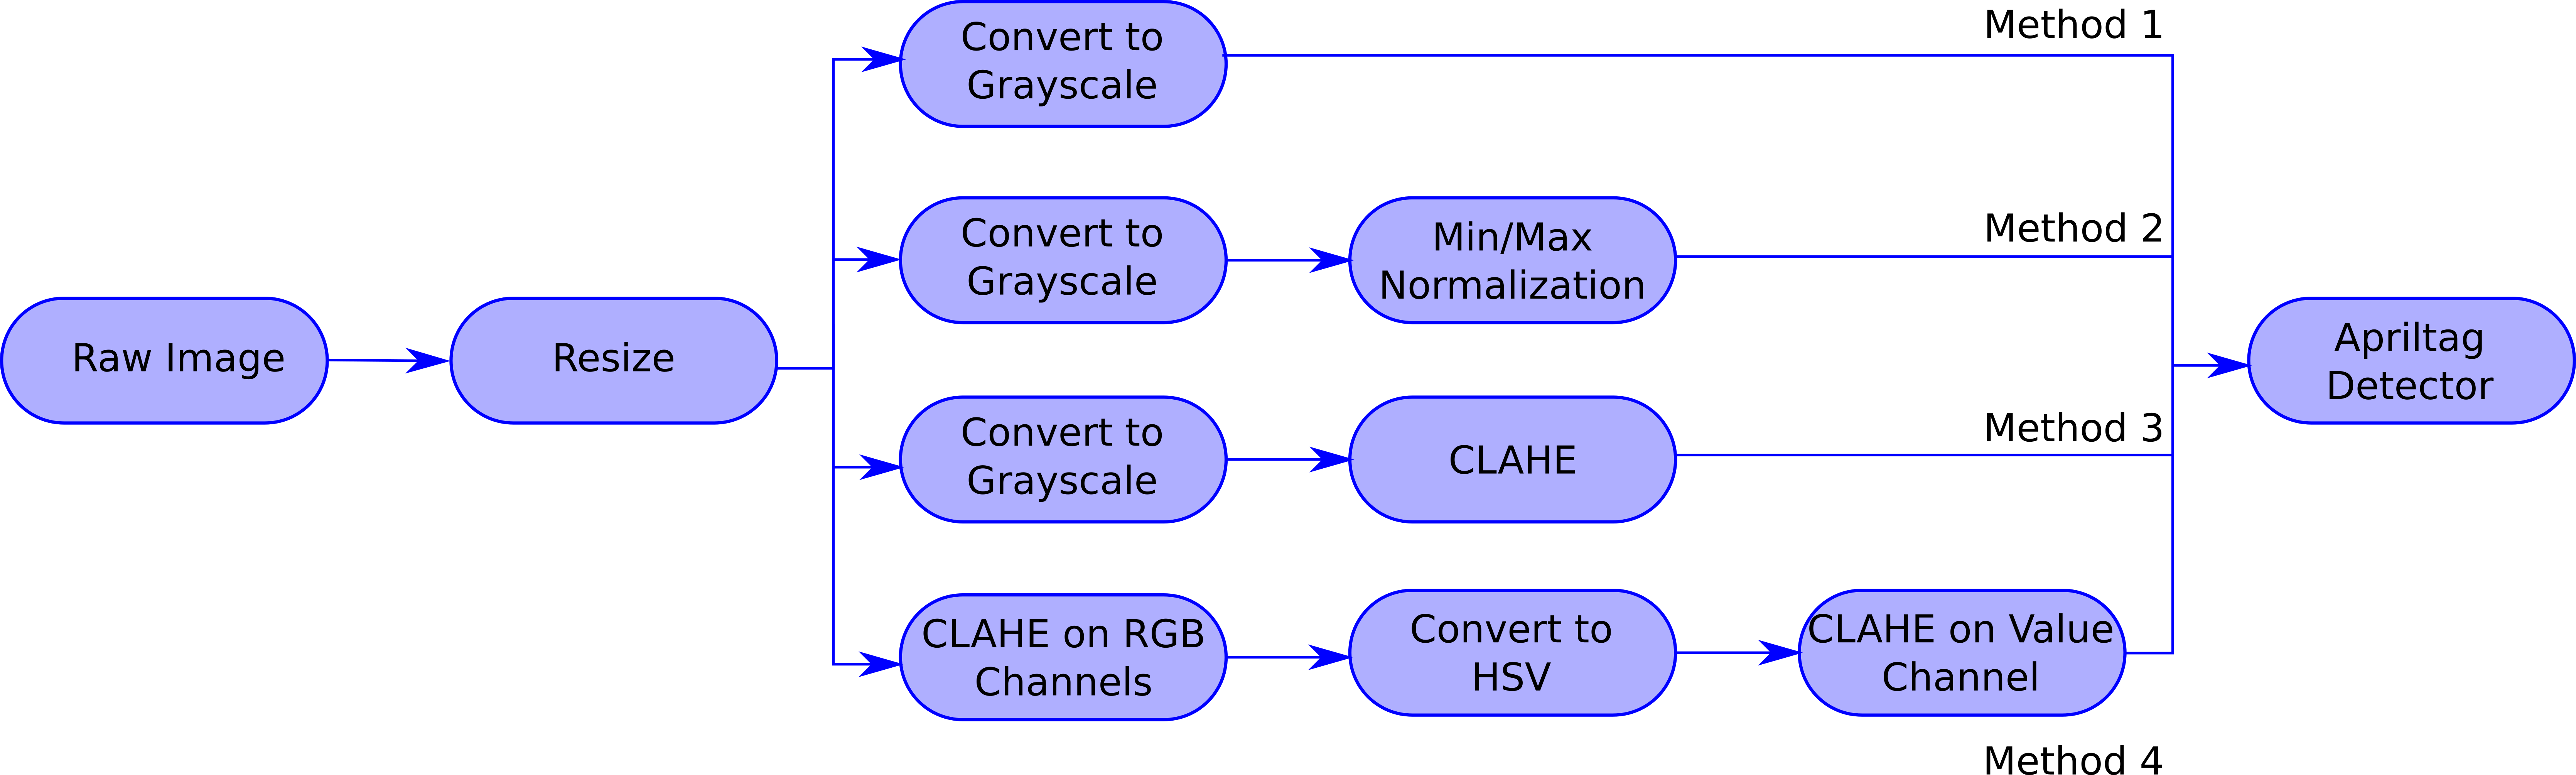
\includegraphics[width=0.49\textwidth]{./fig/processing_flow2.png}
    \caption{Data flow for each method.}
    \label{fig:methods_flow}
\end{figure}


\subsection{Visual Servoing}

On a different day, in order to evaluate the improvement of a visual servoing
task, the vehicle was submitted to a visual servoing under both conditions:
mission with the pre-processing layer and mission without any pre-processing,
and performance of both missions were then compared.

\section{Results and Discussion} \label{sec:results}

The results of the marker detector running through a camera log file with 32613
frames are here shown. It is important to remark that not all the frames
contained a visible marker. Figure \ref{fig:detection_rate} shows the detection
rate of the markers under different pre-processing algorithms and with
different image scales. 

\begin{figure}[!ht]
	\centering
    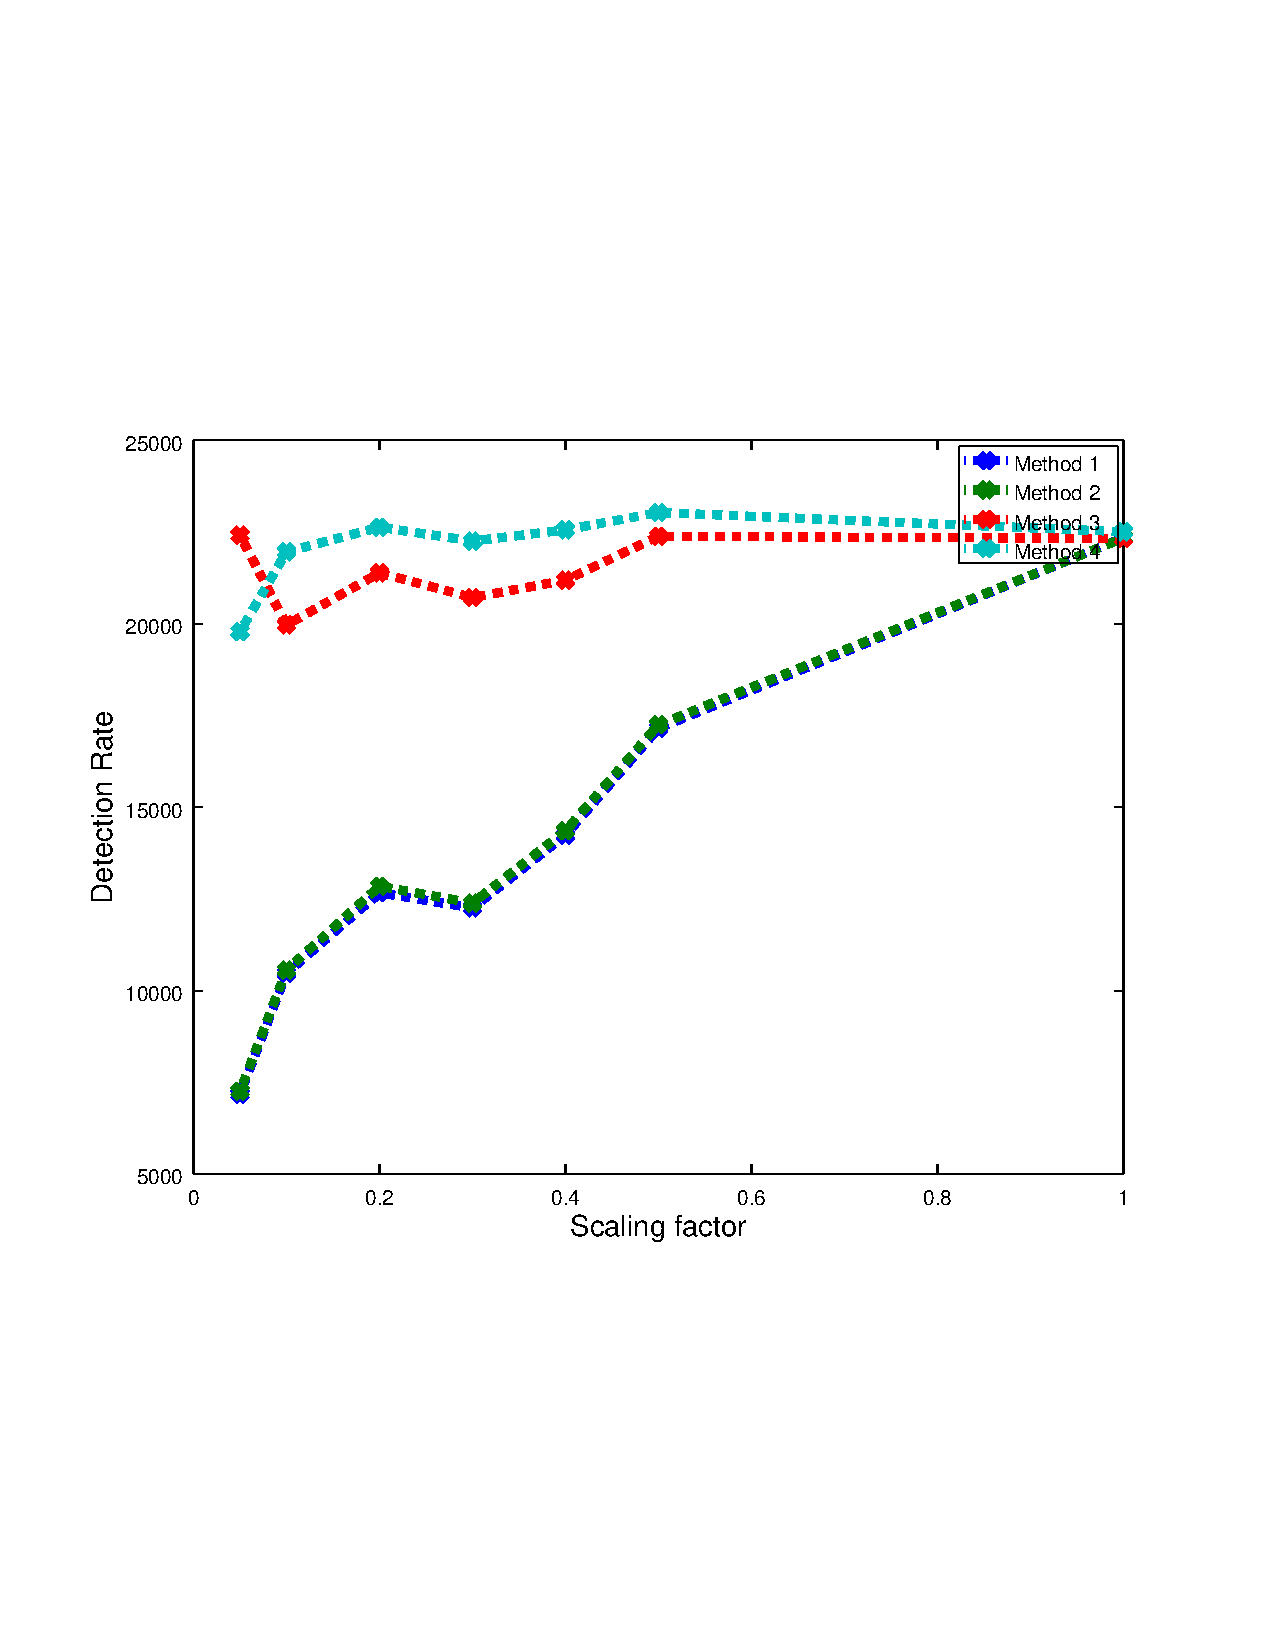
\includegraphics[width=0.4\textwidth, trim={1.6cm 6.9cm 2.3cm 6.7cm}]{./fig/detection_rate.pdf}
    \caption{Relation between detection rate, pre-processing method and image size}
	\label{fig:detection_rate}
\end{figure}

From Figure \ref{fig:detection_rate}, one can see that the frames without any
pre-processing increases the detection rate as long as the image size is bigger.
The normalized image does not show significant change when compared to the
baseline. This behavior is similar for all image resolutions.

On the other hand, it is possible to see on the graph that both Method 3 and
Method 4 surpass the firsts two. In addition, Method 4 presents better performance
than Method 3. Interestingly, neither of these two methods showed dependency to
the scales as much as Methods 1 and 2. Both methods detect more than
20000 frames for all sizes, while the Methods 1 and 2 only achieved this at
full image. 

As already mentioned, the detection rate is not the only important factor since
visual servoing missions are also affected by detection time. Thus, Figure
\ref{fig:processing_time} shows the required processing time for detection of
the studied methods.

\begin{figure}[!ht]
	\centering
    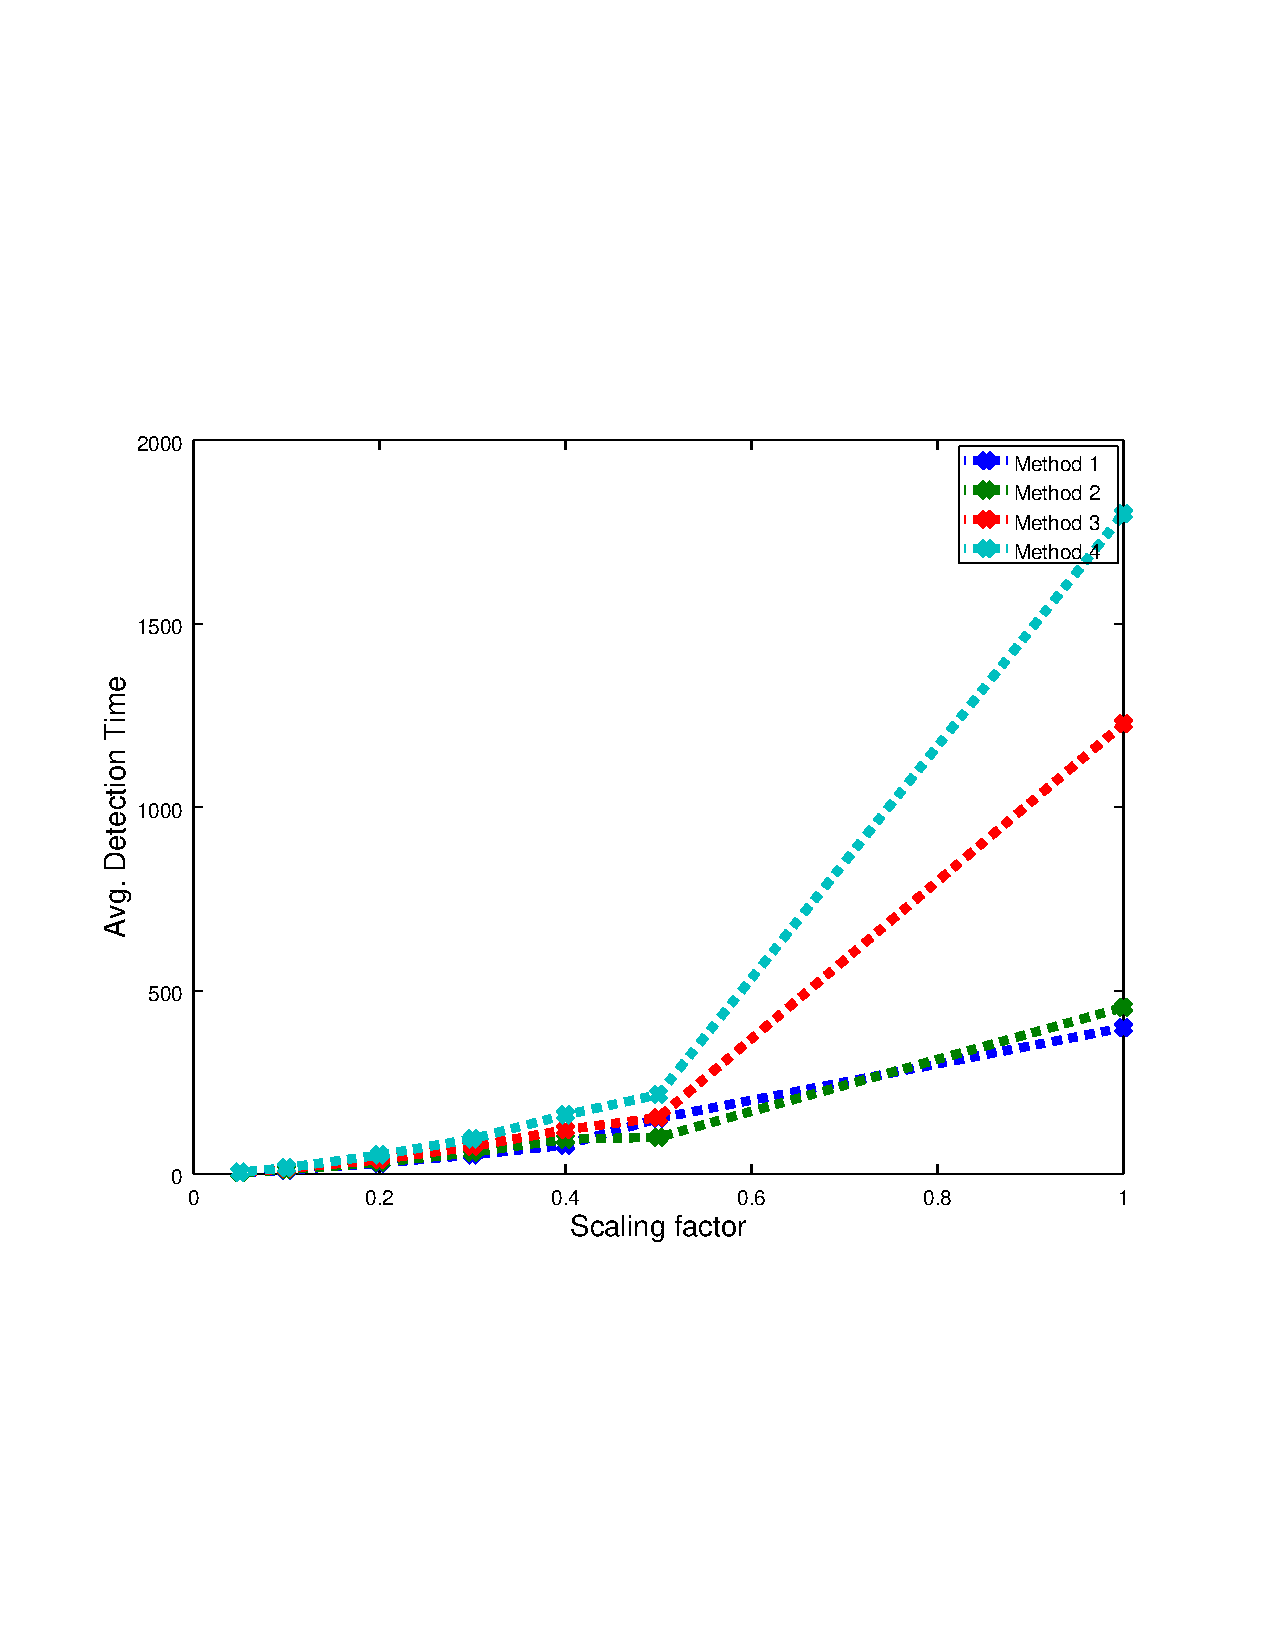
\includegraphics[width=0.4\textwidth, trim={1.6cm 6.9cm 2.3cm 6.7cm}]{./fig/detection_time.pdf}
    \caption{Relation between average processing time, pre-processing method and image size}
	\label{fig:processing_time}
\end{figure}

As expected, processing time increases with image size. Since Method 1
does not have a pre-processing stage, it has the fastest detection time. Method
2 is the second fastest, followed by Method 3 and Method 4, respectively. 

In terms of detection rate, it is possible to see that Methods 3 and 4
surmount Methods 1 and 2.  A closer look on these methods gives us Table
\ref{tab:meth_comp}, which compares Methods 3 and 4.

\begin{table}[]
\centering
\caption{Detection rate and time of Method 4 relatively to Method 3}
\label{tab:meth_comp}
\begin{tabular}{l|ccccccc|}
\cline{2-8}
                                                                                              & \multicolumn{7}{c|}{\textbf{Scale}}                                                                                                                                                   \\
                                                                                              & \textbf{0.05}              & \textbf{0.1}              & \textbf{0.2}              & \textbf{0.3}              & \textbf{0.4}              & \textbf{0.5}              & \textbf{1.0} \\ \hline
\multicolumn{1}{|l|}{\textbf{\begin{tabular}[c]{@{}l@{}}Detection \\ Rate (\%)\end{tabular}}} & \multicolumn{1}{c|}{-11,7} & \multicolumn{1}{c|}{10,0} & \multicolumn{1}{c|}{5,8}  & \multicolumn{1}{c|}{7,4}  & \multicolumn{1}{c|}{6,5}  & \multicolumn{1}{c|}{2,9}  & 0.82      \\ \hline
\multicolumn{1}{|l|}{\textbf{\begin{tabular}[c]{@{}l@{}}Detection \\ Time (\%)\end{tabular}}} & \multicolumn{1}{c|}{13,5}  & \multicolumn{1}{c|}{16,7} & \multicolumn{1}{c|}{32,9} & \multicolumn{1}{c|}{28,1} & \multicolumn{1}{c|}{33,4} & \multicolumn{1}{c|}{40,7} & 46.62       \\ \hline
\end{tabular}
\end{table}

Images with small resolution affect pose estimation accuracy. Thus, we
will use the highest resolution in which we have a reasonable time for the
visual servoing task for comparison purposes. In this case, we decided to use the scale
factor of 0.4, which causes the image resolution to be 816x816 and feed the
visual controller at 6.25Hz.

At this scale factor, Method 4 improves the detection rate in 6.45\%, but it
comes with the cost of an increase of 33.44\% in average detection time. Thus,
we prefer to use Method 3 instead of Method 4.

\subsection{Visual servoing performance}

The vehicle was moved to the front of the marker and waited for a stable
detection before starting the visual servoing task. However, due to the poor
visibility on the day, the Apriltags marker was not able to detect any marker,
which invalidated the visual servoing without any pre-processing. After it was
able to apply Method 3, the marker detection started and allowed a visual
servoing mission. The results of the visual servoing are shown in Figures
\ref{fig:vs_surge} to \ref{fig:vs_yaw}.

This clearly shows the improvement caused by image treatment before
running the visual servoing mission. In that case, specifically, the visual
servoing was not be possible by using only the grayscale image. So it improved
from a state of no-operation to a regular mission.

\begin{figure}[!ht]
	\centering
    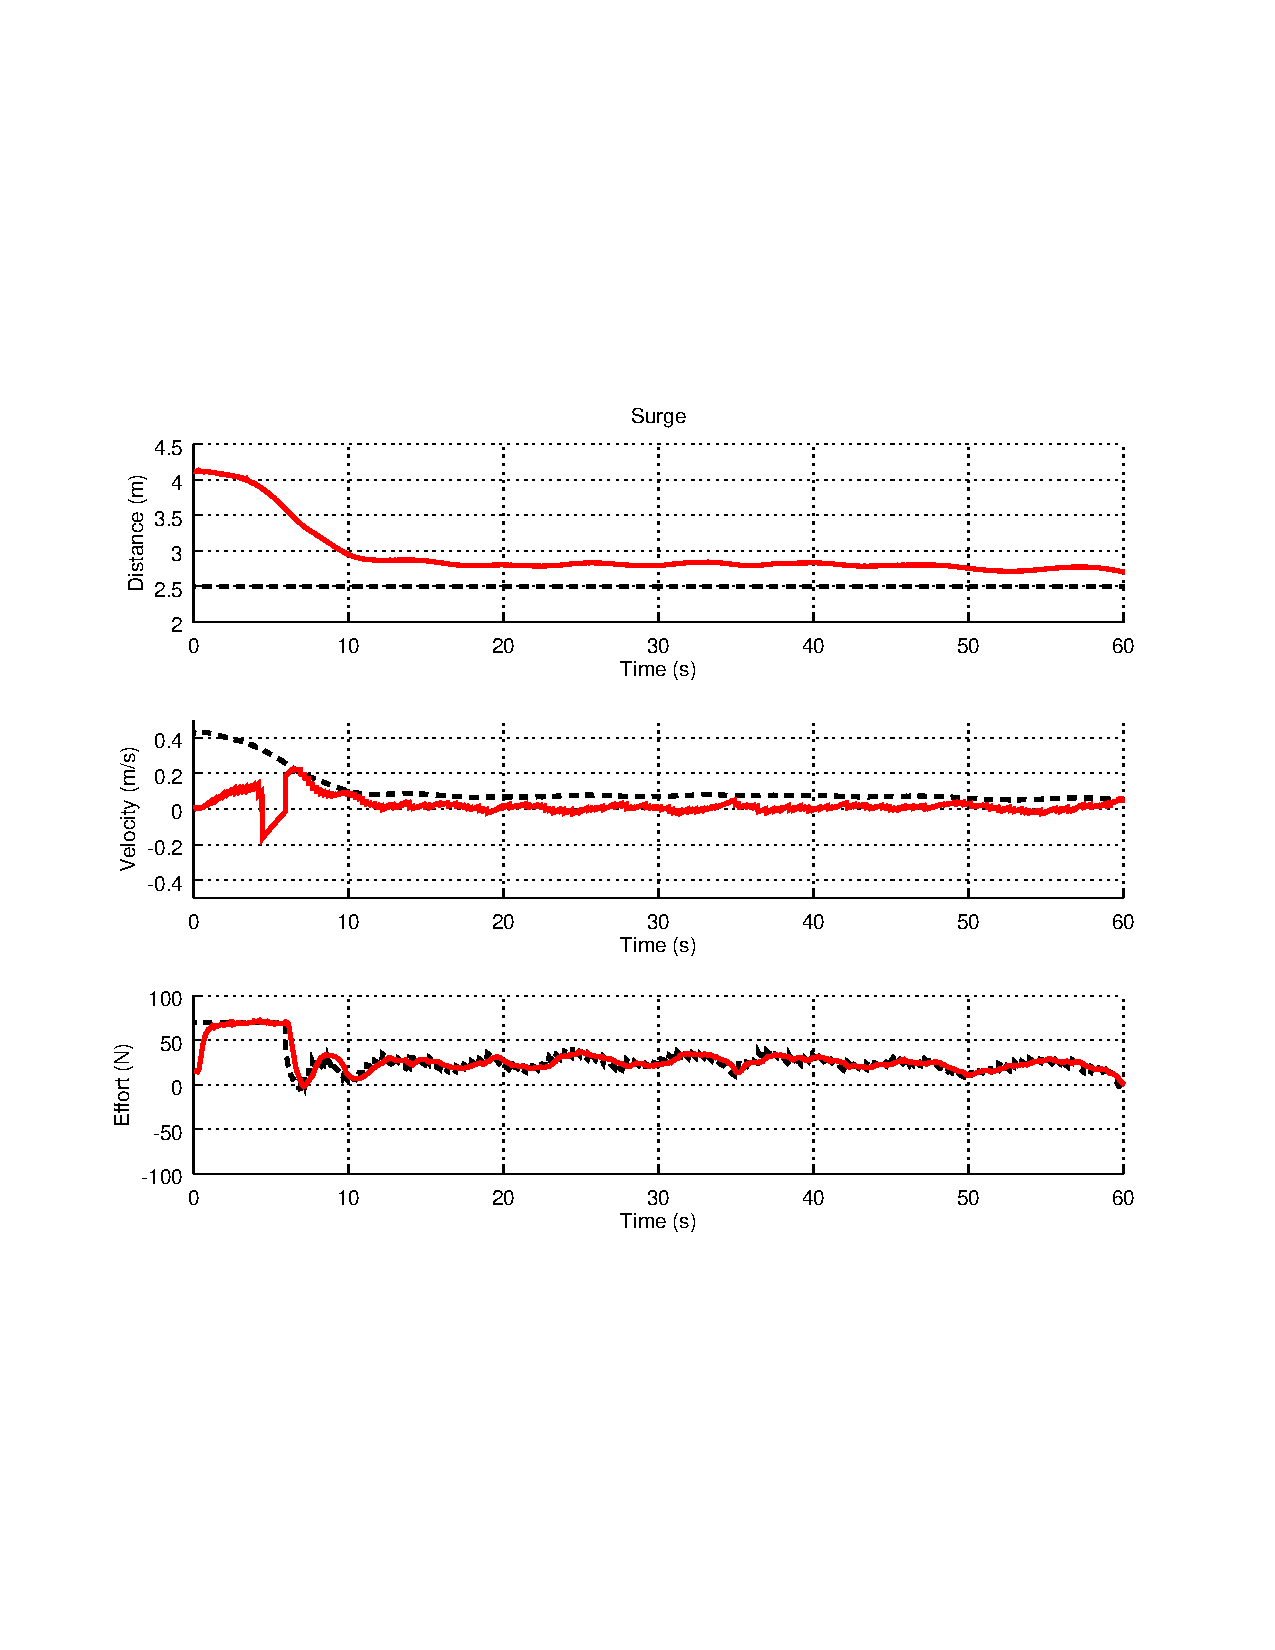
\includegraphics[width=0.49\textwidth, trim={1.6cm 6.9cm 2.3cm 6.7cm}]{./fig/vs_surge.pdf}
    \caption{Visual servoing performance in surge}
	\label{fig:vs_surge}
\end{figure}
\begin{figure}[!ht]
	\centering
    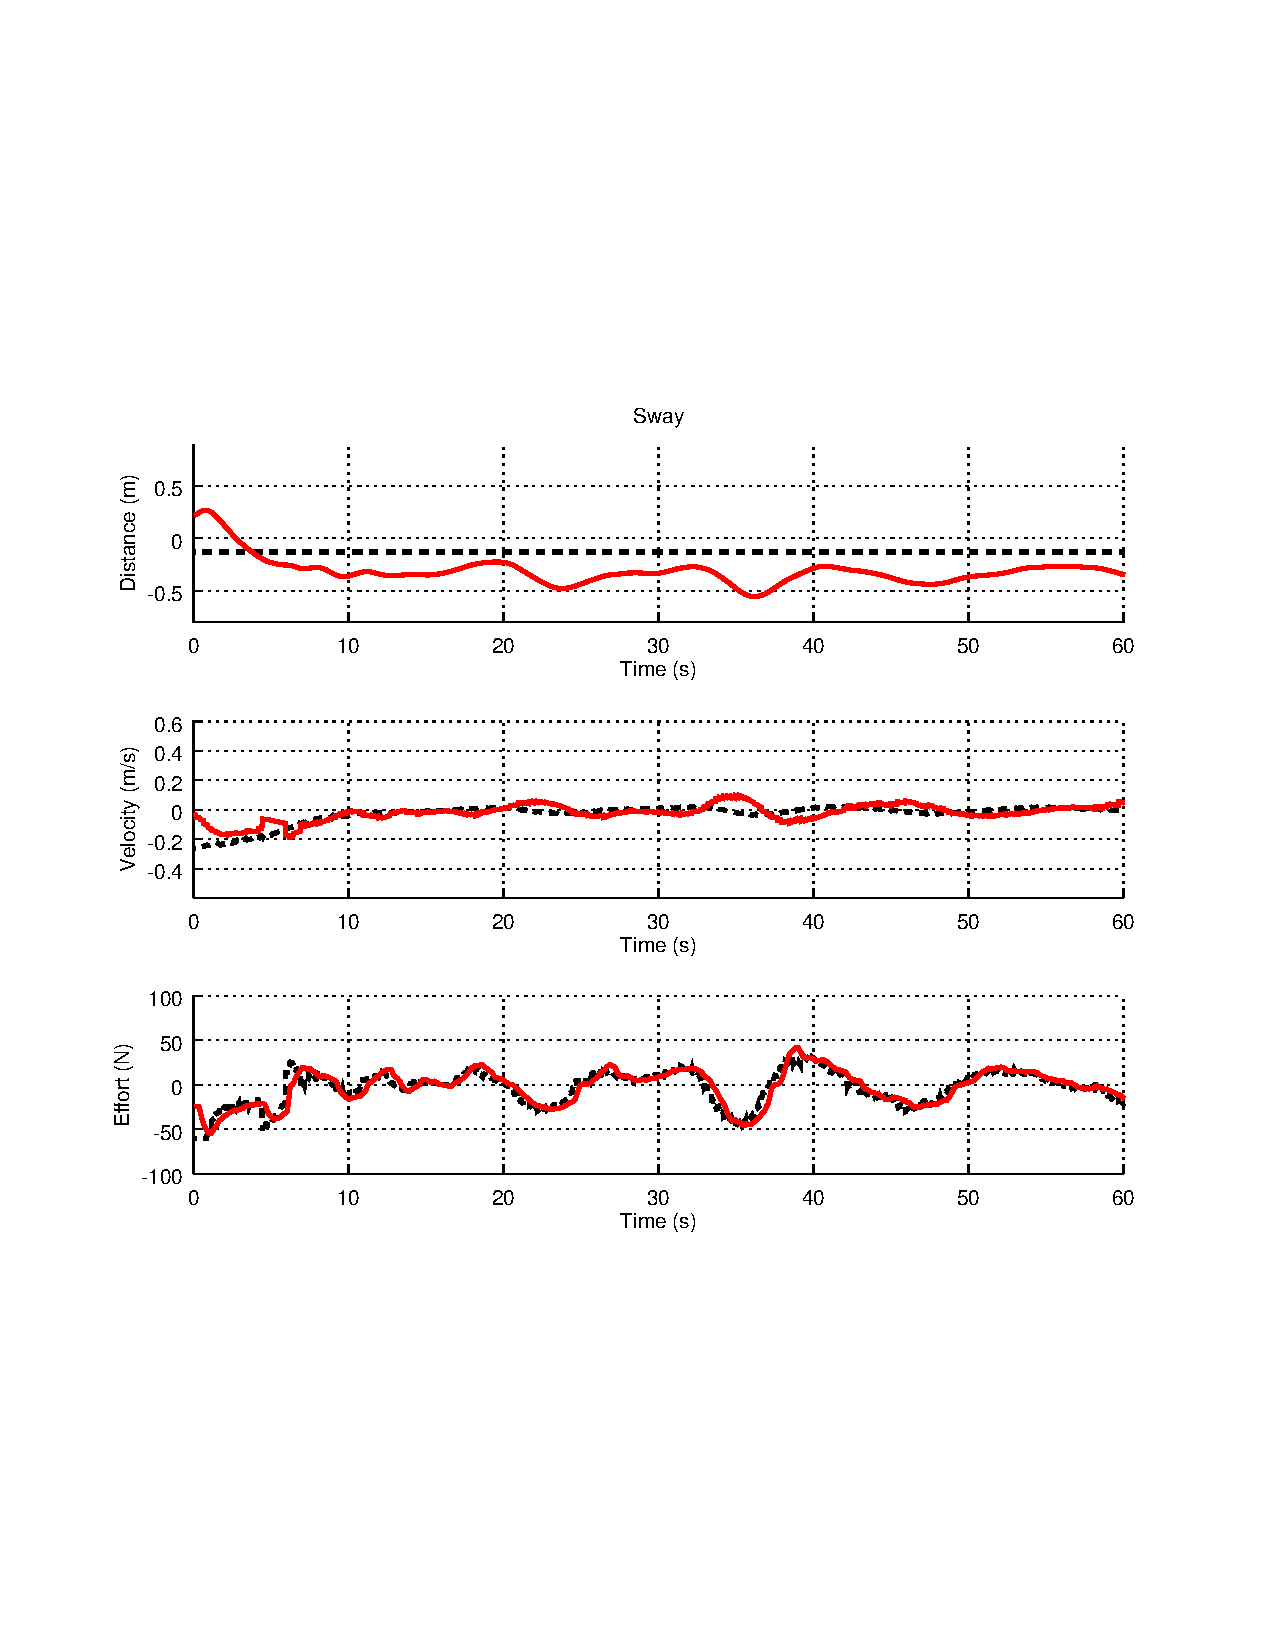
\includegraphics[width=0.49\textwidth, trim={1.6cm 6.9cm 2.3cm 6.7cm}]{./fig/vs_sway.pdf}
    \caption{Visual servoing performance in sway}
	\label{fig:vs_sway}
\end{figure}
\begin{figure}[!ht]
	\centering
    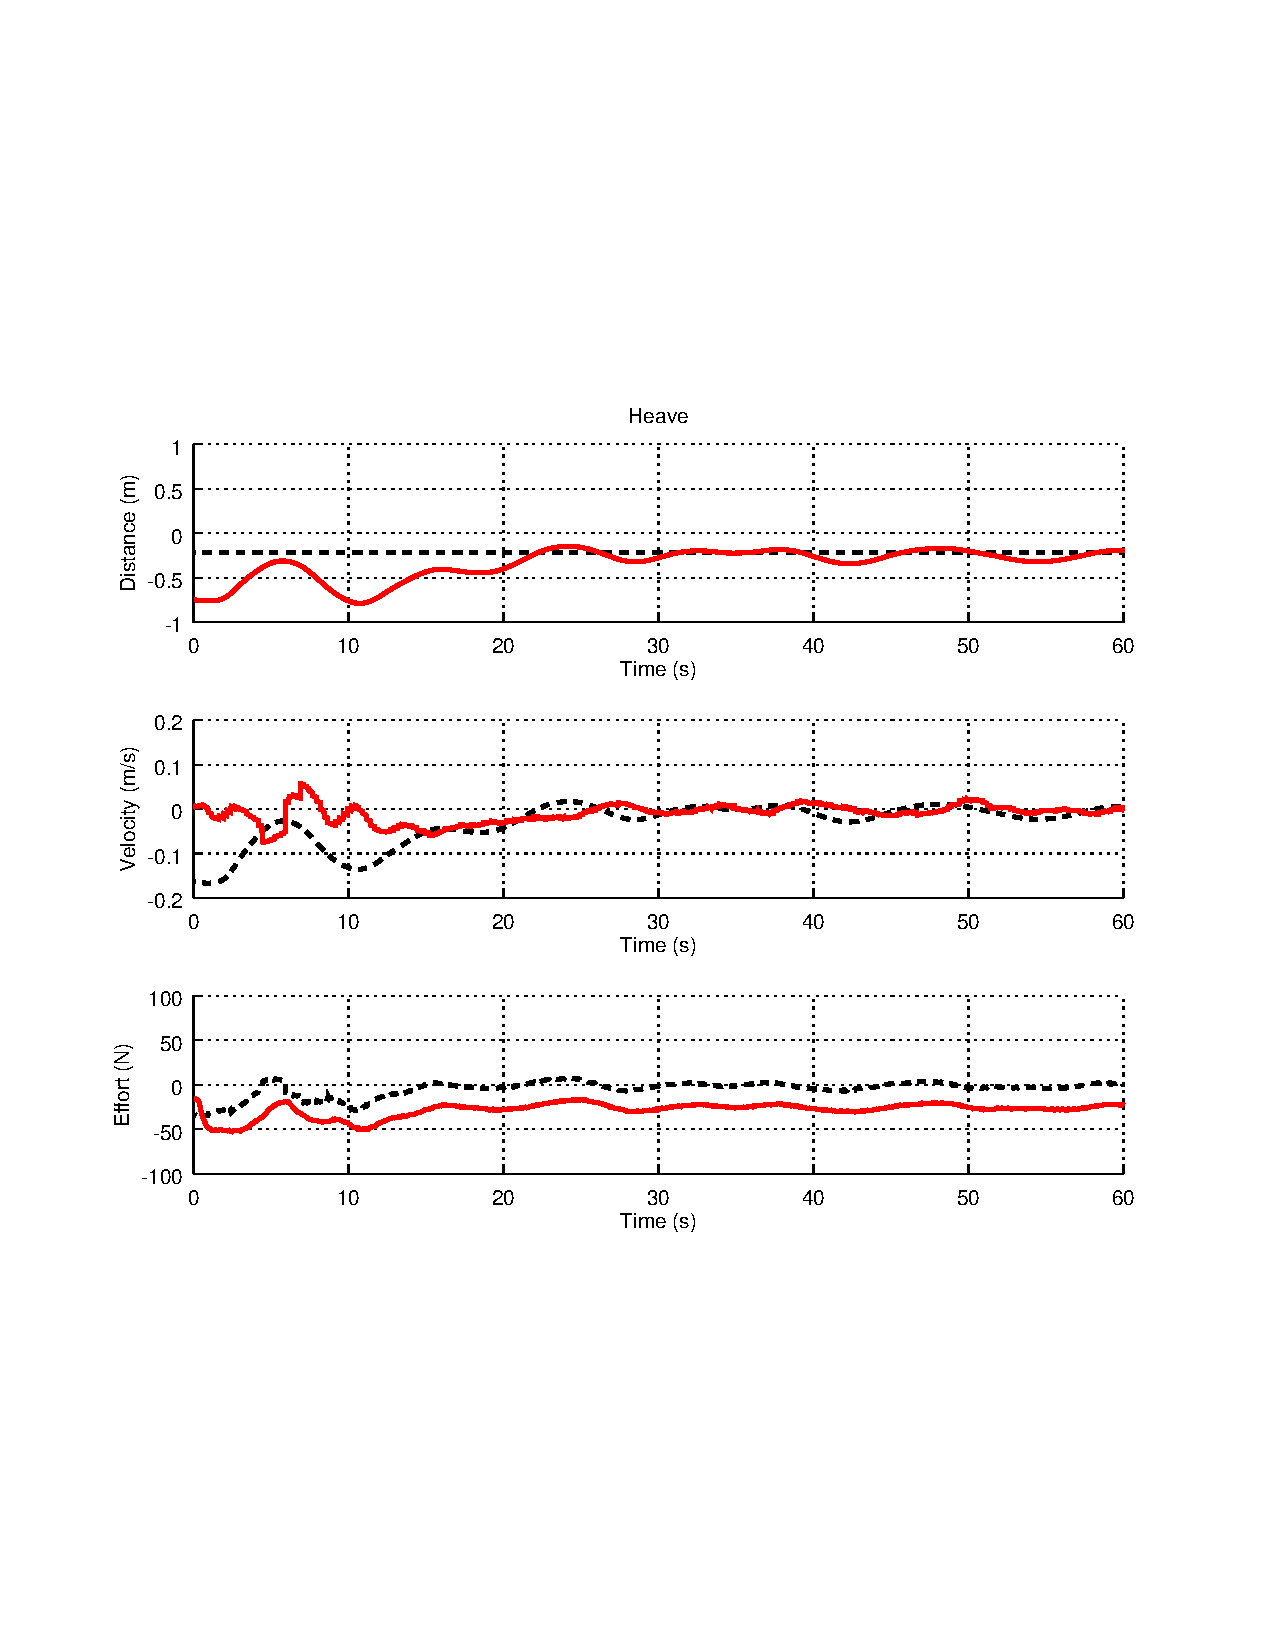
\includegraphics[width=0.49\textwidth, trim={1.6cm 6.9cm 2.3cm 6.7cm}]{./fig/vs_heave.pdf}
    \caption{Visual servoing performance in heave}
	\label{fig:vs_heave}
\end{figure}

\begin{figure}[!ht]
	\centering
    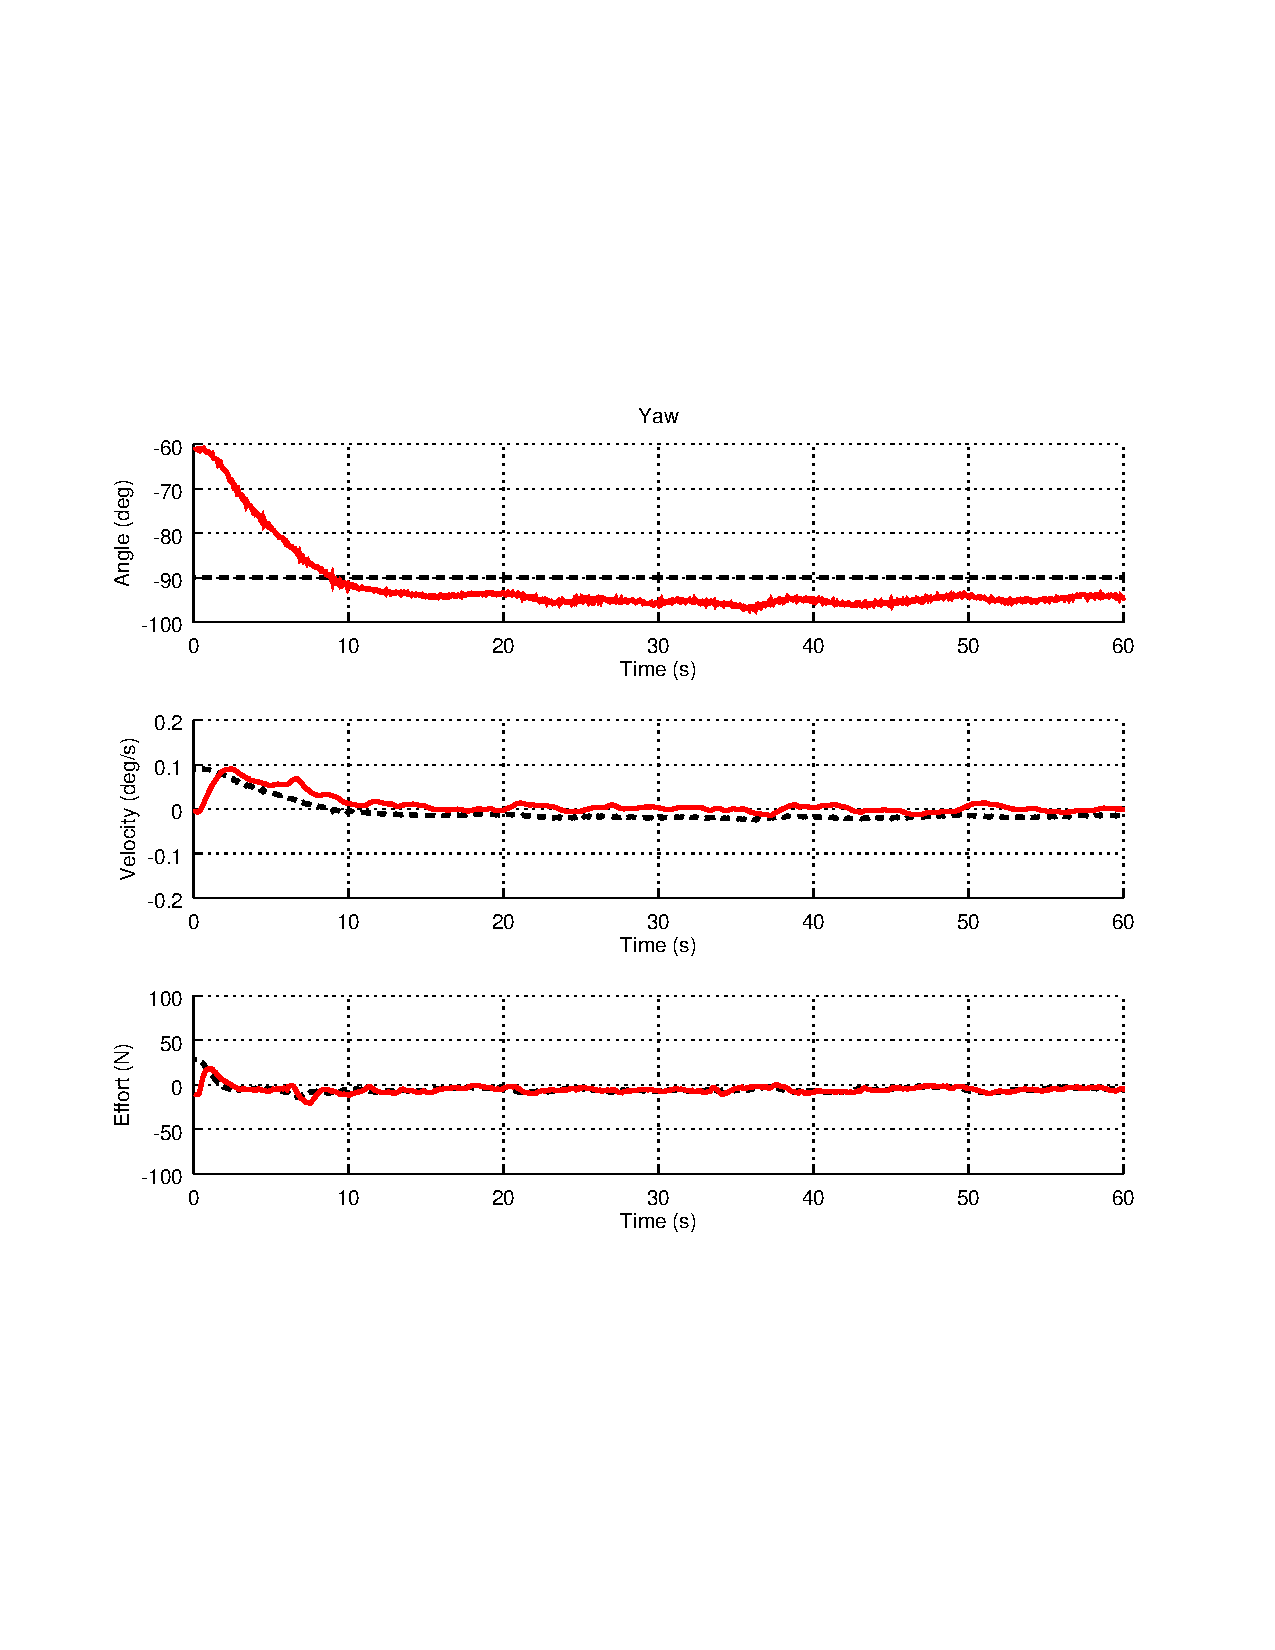
\includegraphics[width=0.49\textwidth, trim={1.6cm 6.9cm 2.3cm 6.7cm}]{./fig/vs_yaw.pdf}
    \caption{Visual servoing performance in yaw}
	\label{fig:vs_yaw}
\end{figure}

Later, the methods were once again applied to a log data. The results are shown
in Figures \ref{fig:detection_rate2} and \ref{fig:detection_time2}. It shows
the inability of the marker detector to detect markers with Method 1 and
Method 2. On the other hand, Methods 3 and 4 were able to detect most of the
8956 frames contained in the log file. 

\begin{figure}[!ht]
	\centering
    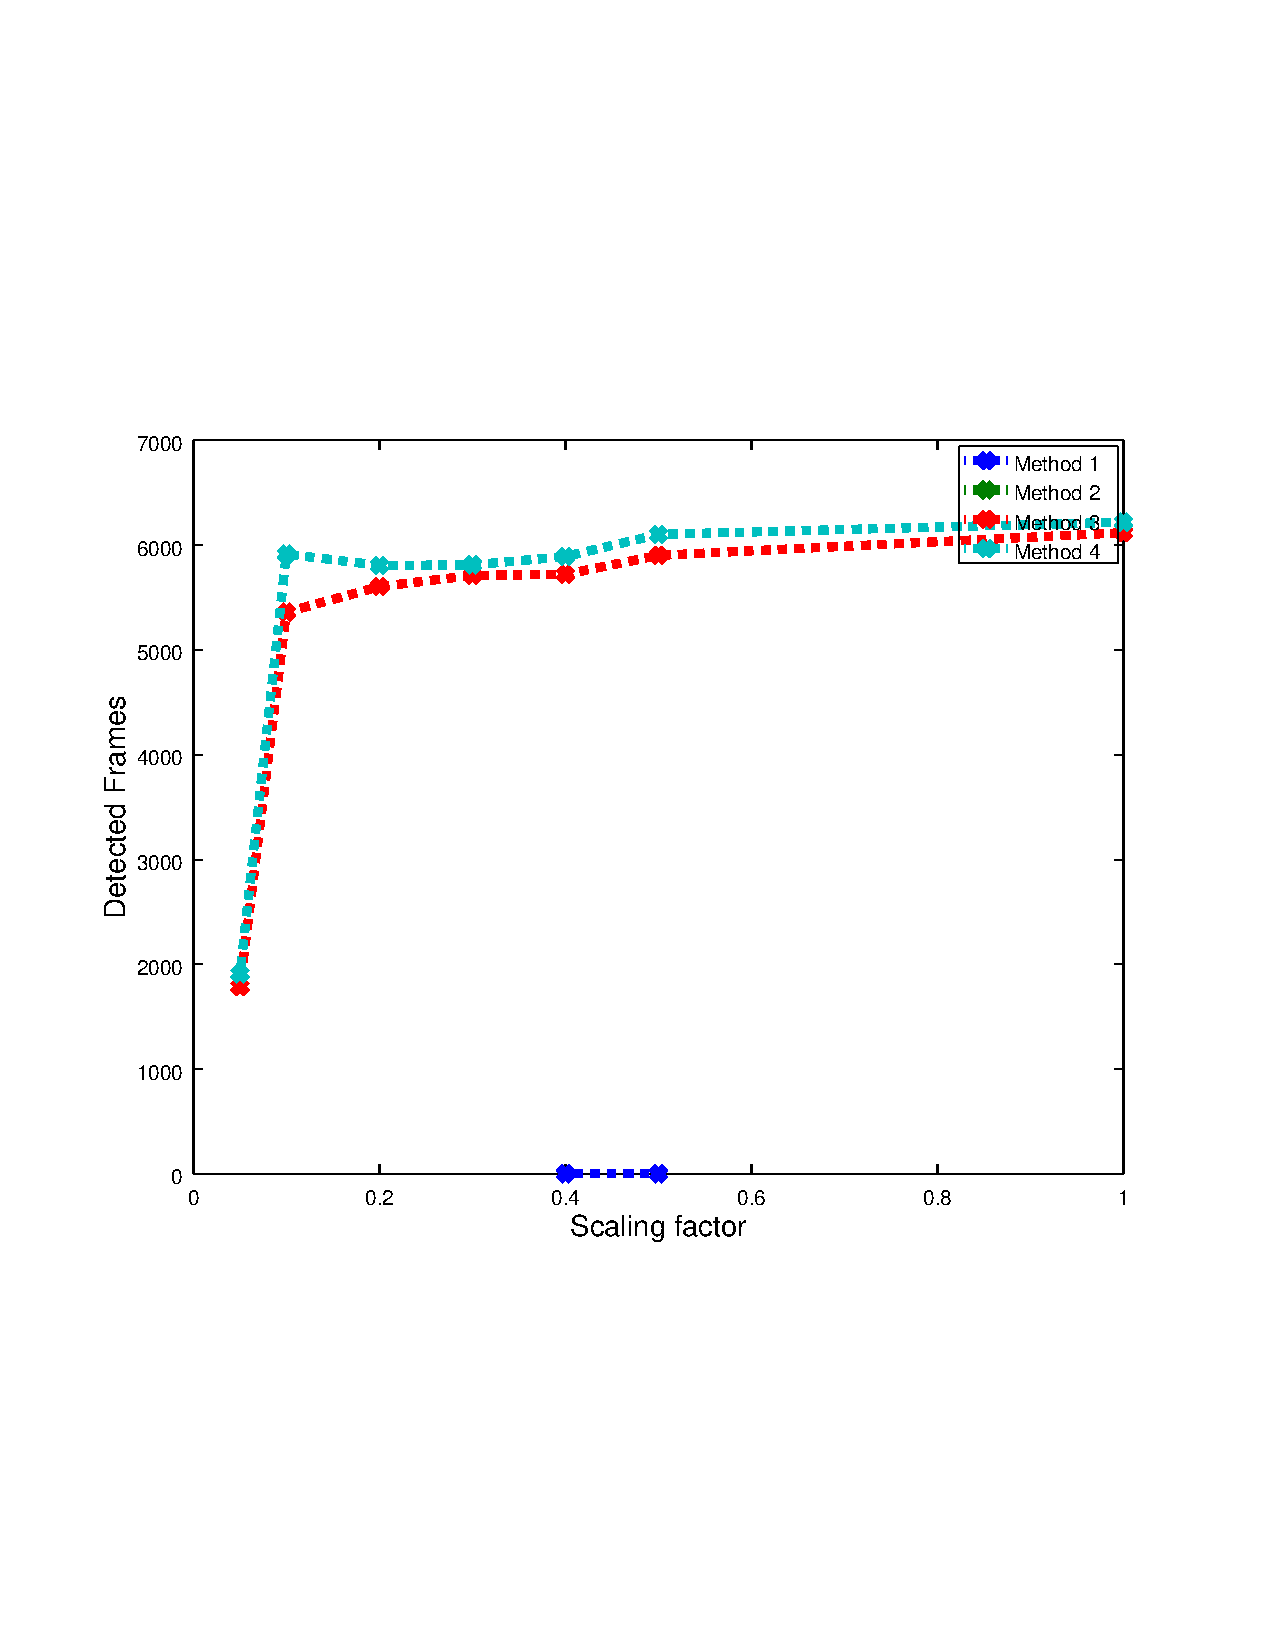
\includegraphics[width=0.4\textwidth, trim={1.6cm 6.9cm 2.3cm 6.7cm}]{./fig/detection_rate2.pdf}
    \caption{Relation between detection rate, pre-processing method and image size}
	\label{fig:detection_rate2}
\end{figure}

\begin{figure}[!ht]
	\centering
    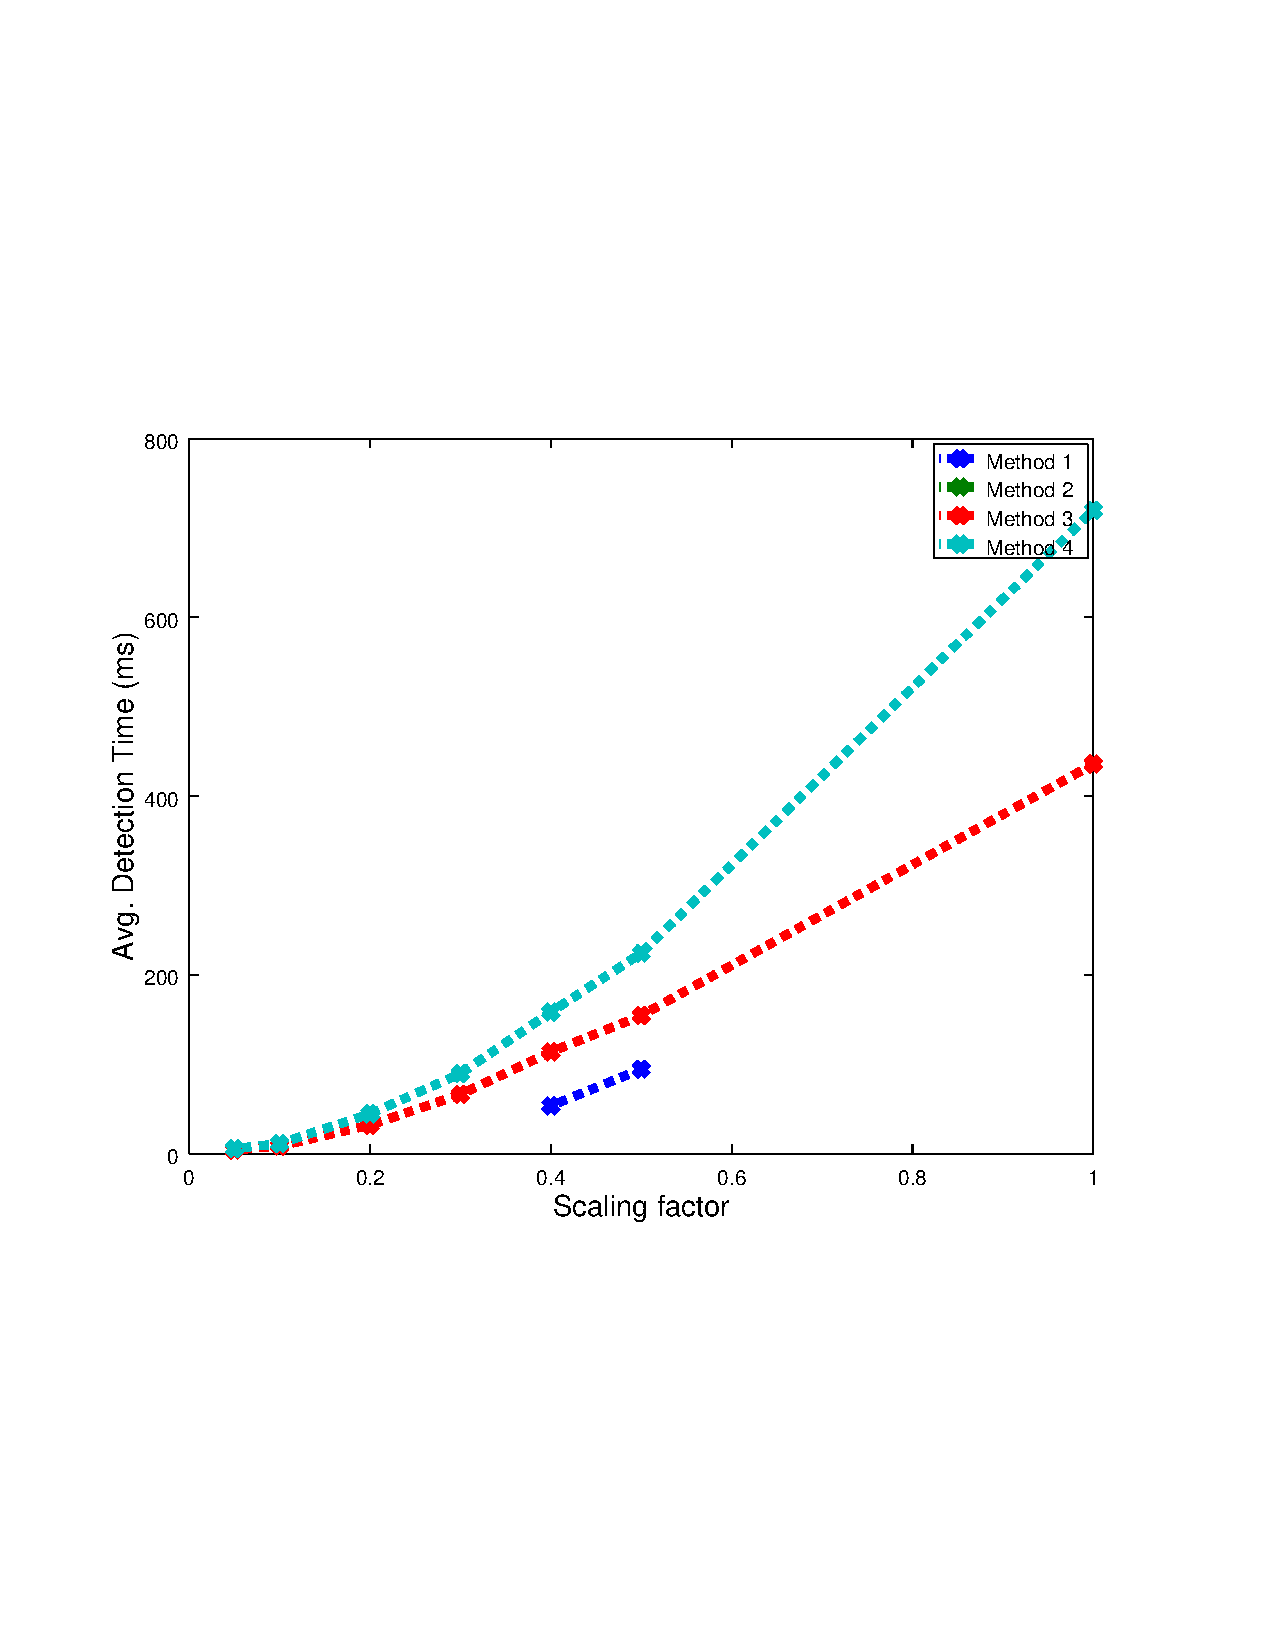
\includegraphics[width=0.4\textwidth, trim={1.6cm 6.9cm 2.3cm 6.7cm}]{./fig/detection_time2.pdf}
    \caption{Relation between average processing time, pre-processing method and image size}
	\label{fig:processing_time2}
\end{figure}

\section{Conclusion} \label{sec:concl}

On this paper we briefly presented the concepts and challenges of underwater
image formation. It also was presented three methods to improve the underwater
image aiming to increase the detection rate of artificial fiducial markers.
Since the purpose of the detection is to feed a visual controller for visual
servoing task, the time for detection is also observed.

The results showed that simply applying a local contrast enhancement on the
image increases significantly the detection rate. A method based on Iqbal's
paper is also applied. Although the Iqbal's based-method increases the
detection rate, the processing time increases in a higher proportion, which
caused its use not be the preferable for the visual servoing, when compared to
Method 3.

We also have seen that, due to the underwater image quality, the marker
detector was not able to feed the visual controller using raw image. On the
other hand, using Method 3, the marker detector found several images and
performed visual servoing normally. This result shows the proposed methods not
only increases the visual controller frequency, by the improvement of the
detection rate, but also makes the visual servoing possible when the image
quality is not favorable.

% use section* for acknowledgment
\section*{Acknowledgment}

The authors would like to thank all involved colleagues at SENAI CIMATEC for
the support. This work is part of the FlatFish project, which is funded by
Shell, the Brazilian Industrial Research and Innovation Corporation (EMBRAPII)
and the Brazilian National Agency of Petroleum (ANP).

% trigger a \newpage just before the given reference
% number - used to balance the columns on the last page
% adjust value as needed - may need to be readjusted if
% the document is modified later
%\IEEEtriggeratref{8}
% The "triggered" command can be changed if desired:
%\IEEEtriggercmd{\enlargethispage{-5in}}

% references section

% can use a bibliography generated by BibTeX as a .bbl file
% BibTeX documentation can be easily obtained at:
% http://mirror.ctan.org/biblio/bibtex/contrib/doc/
% The IEEEtran BibTeX style support page is at:
% http://www.michaelshell.org/tex/ieeetran/bibtex/
\bibliographystyle{IEEEtran}
% argument is your BibTeX string definitions and bibliography database(s)
\bibliography{IEEEabrv,./bib/ref.bib}

% that's all folks
\end{document}
